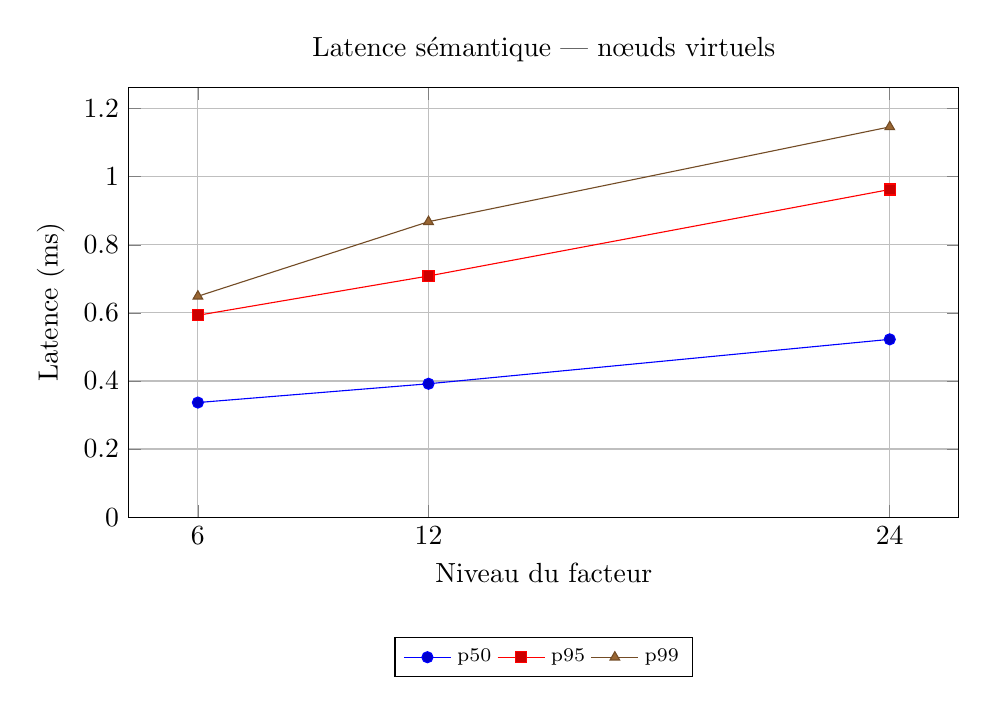
\begin{tikzpicture}
\begin{axis}[width=\linewidth,
height=0.58\linewidth,
title={Latence sémantique — nœuds virtuels},
xlabel={Niveau du facteur},
ylabel={Latence (ms)},
grid=major,
legend style={font=\scriptsize,at={(0.5,-0.28)},anchor=north,legend columns=3},
xtick={6.0,12.0,24.0},
ymin=0]
\addplot+[mark=*] coordinates {(6.0,0.3365545) (12.0,0.391725) (24.0,0.522252)};
\addlegendentry{p50}
\addplot+[mark=square*] coordinates {(6.0,0.5928659) (12.0,0.70835425) (24.0,0.96242995)};
\addlegendentry{p95}
\addplot+[mark=triangle*] coordinates {(6.0,0.64883945) (12.0,0.86791226) (24.0,1.14638757)};
\addlegendentry{p99}
\end{axis}
\end{tikzpicture}
